\section{Introducción}

\begin{frame}{Introducción}
	\begin{block}{Google Chromecast}
	Google Chromecast es un dispositivo de reproducción multimedia. Se conecta a una televisión o monitor vía HDMI y hace streaming mediante Wi-Fi.
	El contenido puede alojarse en un dispositivo conectado a una red local o en un sevidor externo.
	\end{block}
	
	\begin{block}{Streaming}
	Utiliza el software propietario Google Cast, controlando la reproducción multimedia en un receptor desde uno o varios dispositivos locales.
	Es compatible con Android, iOS, Chrome OS y aplicaciones de
	Google Chrome.
	\end{block}
\end{frame}


\begin{frame}{Tipos}
	\begin{exampleblock}{Vídeo y audio}
		\begin{itemize}
			\item Chromecast primera generación
			\item Chromecast segunda generación (compatible Wi-Fi 5GHz)
			\item Chromecast Ultra (reproducción 4k)
		\end{itemize}
	\end{exampleblock}
	
	\begin{exampleblock}{Audio}
		\begin{itemize}
			\item  Chromecast Audio
		\end{itemize}
	\end{exampleblock}
\end{frame}


\begin{frame}{Chromecast primera generación}
	\begin{block}{Hardware}
		\begin{itemize}
			\item 512 MB de Micron DDR3L RAM
			\item 2/4 GB de memoria flash
		\end{itemize}
		Incluye salida HDMI, entrada micro USB para alimentación, un LED que indica el estado del dispositivo y un botón de reset.
	\end{block}
	\begin{figure}[h]
		\centering
		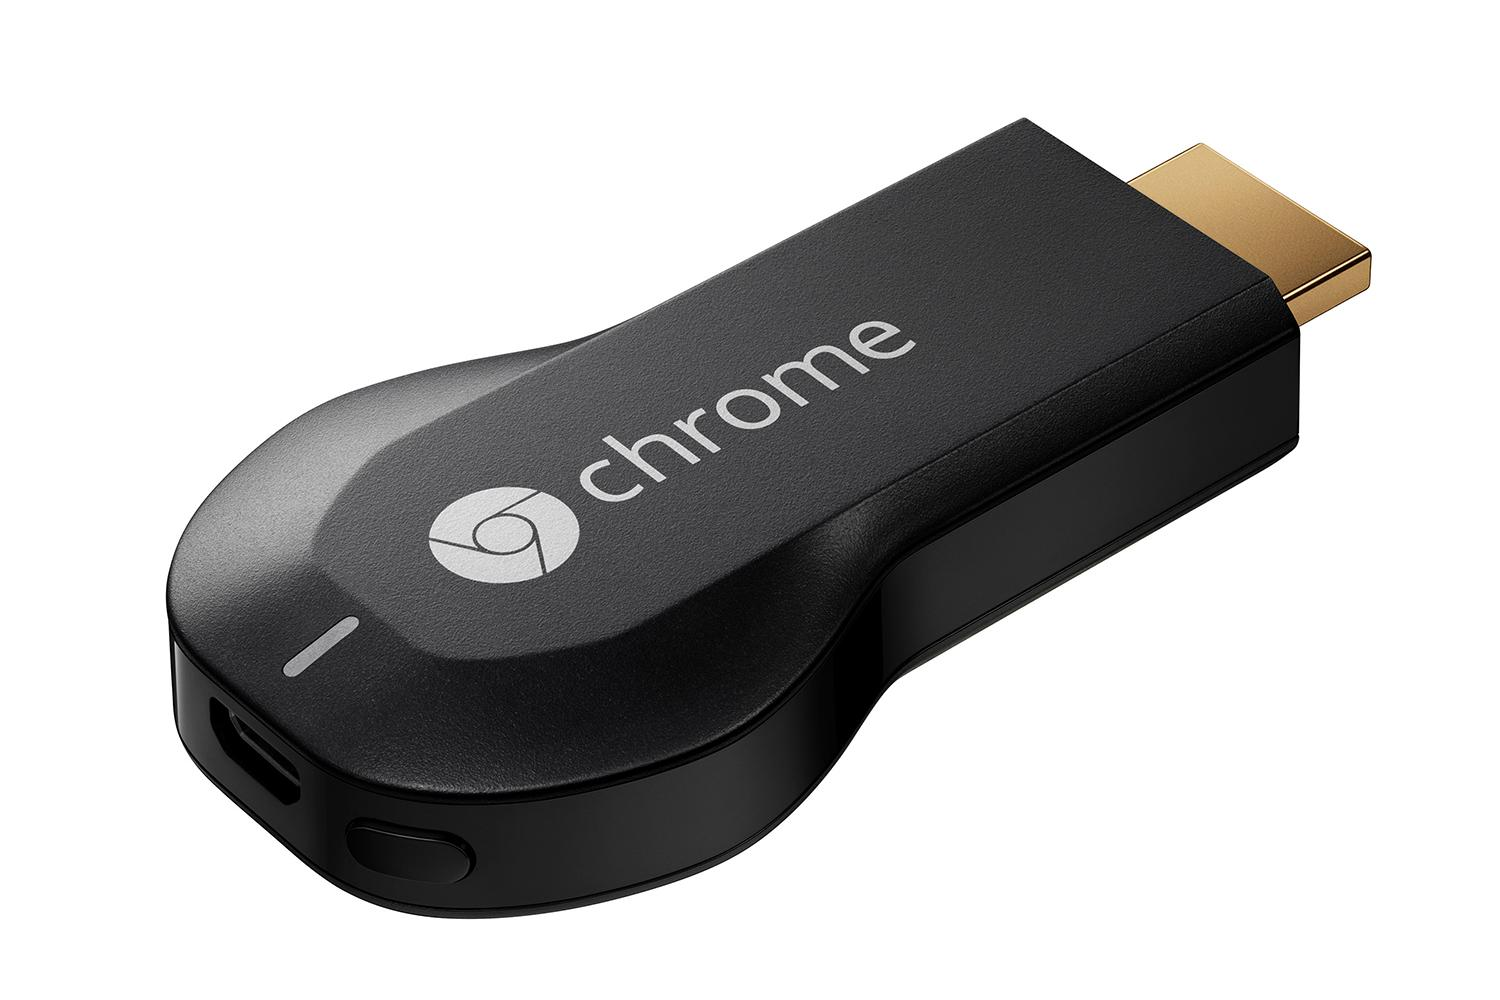
\includegraphics[width=0.55\textwidth]{./Imagenes/chromecast1gen.jpg}
	\end{figure}
\end{frame}


\begin{frame}{Chromecast segunda generación}
	\begin{block}{Diferencias}
		256 MB de memoria flash, procesador con dos núcleos y tres antenas para mejorar la conexión con el router.
	\end{block}
	\begin{figure}[h]
		\centering
		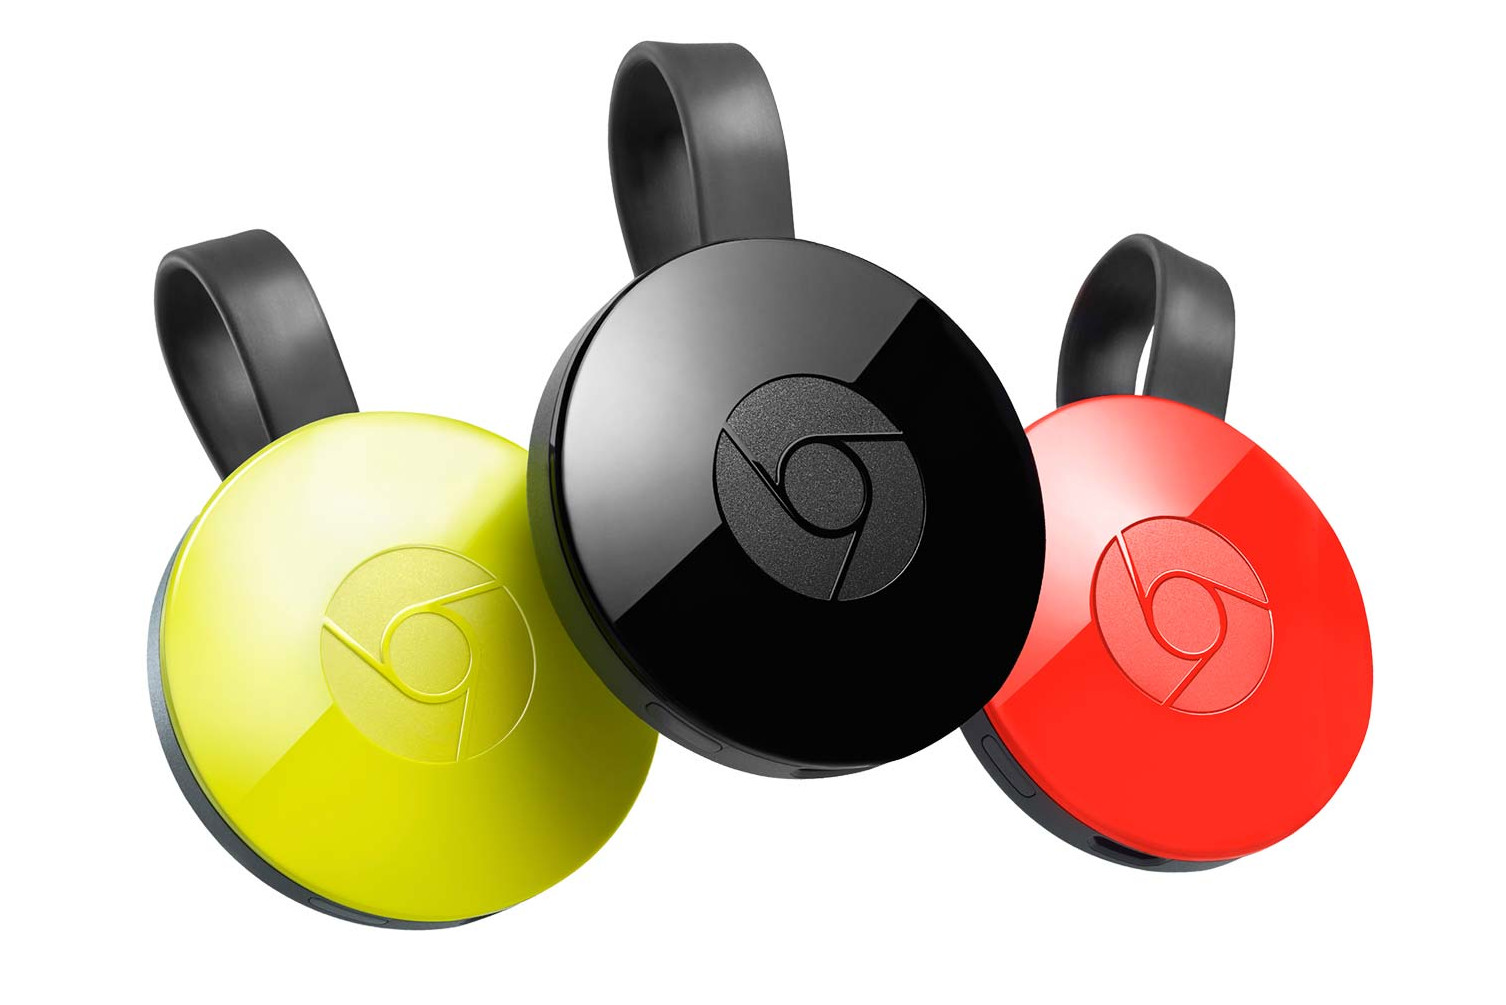
\includegraphics[width=0.75\textwidth]{./Imagenes/chromecast2gen.jpg}
	\end{figure}
\end{frame}


\begin{frame}{Chromecast Audio}
	\begin{block}{Diferencias}
		Salida MiniJack de 3,5mm en lugar del HDMI.
	\end{block}
	
	\begin{figure}[h]
		\centering
		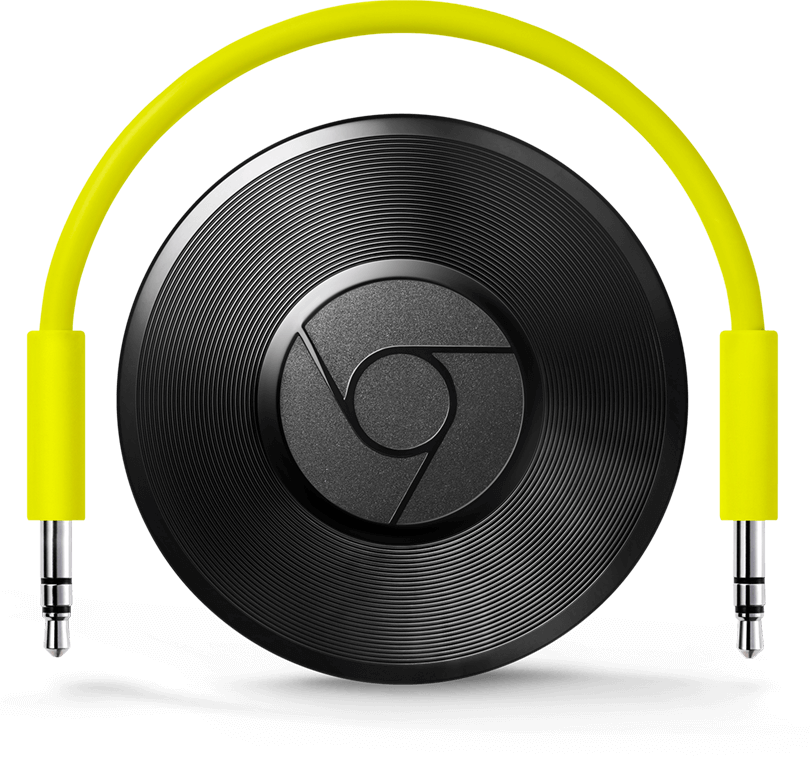
\includegraphics[width=0.45\textwidth]{./Imagenes/chromecastaudio.png}
	\end{figure}
\end{frame}


\begin{frame}{Chromecast Ultra}
	\begin{block}{Diferencias}
		Entrada Ethernet para conexión a Internet.
	\end{block}
	
	\begin{figure}[h]
		\centering
		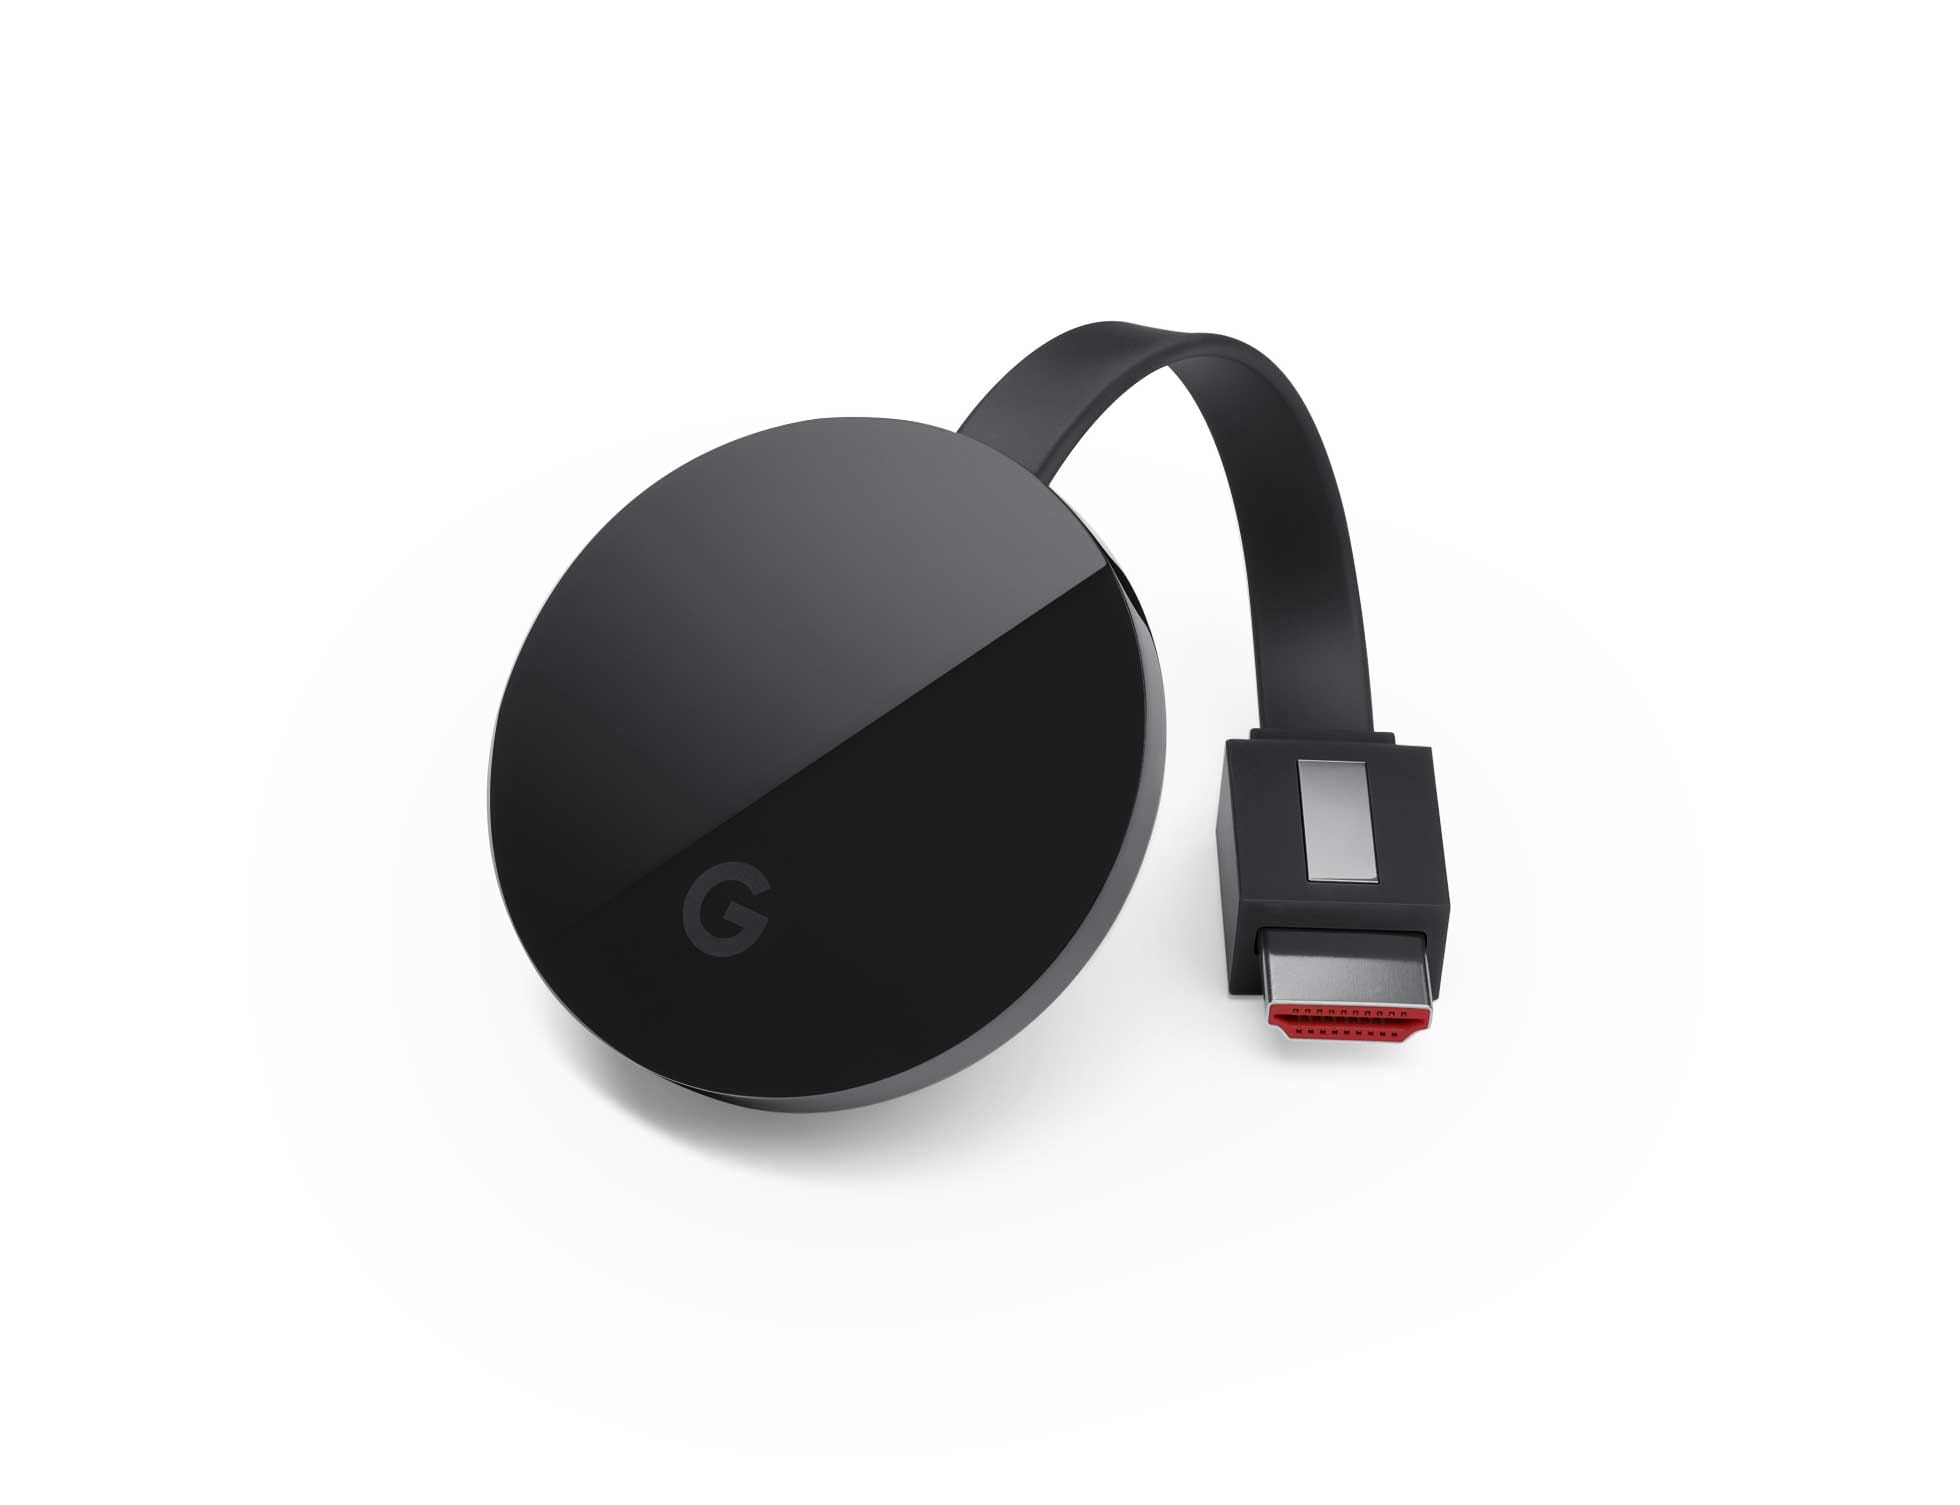
\includegraphics[width=0.5\textwidth]{./Imagenes/chromecast-ultra.jpg}
	\end{figure}
\end{frame}